\chapter{Diversité} \label{ch:DIV}

\section{Mesures et méthodologie}

L'objectif du travail est de quantifier l'impact de la diversité sur la propagation de pandémies. Cette section est dédie à la prise de mesures avec des niveaux de diversité différents et d'en constater les résultats. Afin de ne pas trop complexifier le modèle au-delà des simulations SIR, nous ne modifions que le paramètre de diversité, nombre de mouvements ainsi que la charge virale. D'autres paramètres du modèle pourraient être étudié mais ce chapitre ne les explore pas.\\

La recherche sur la diversité est découpée en trois parties. La première explore l'impact de la diversité sur des simulations à propagation de pandémie rapide. Dans ce cas nous observons donc la réaction de la diversité sur l'immunisation des individus déjà contaminés. La seconde cherche à déterminer le taux de simulations qui développent une pandémie, c'est-à-dire le nombre de simulations qui réussissent ou échouent à développer une pandémie en fonction de la diversité de la population. La troisième tente d'observer des pandémies partielles qui ne parviennent pas à contaminer toute la population.\\


\section{Pandémies totales}

Le premier chapitre est une observation de l'impact de la diversité sur des systèmes de densité $1/16$ au mélange parfait. L'analyse est purement qualitative et permet de visualiser le comportement du mécanisme d'immunisation en fonction du facteur de diversité.\\

L'unique simulation étudié est de taille $1264 \times 1264$ avec une population de $10^5$ individus. La charge virale est définie à $1$ et la diversité est de $4,8,16,32$. Les génomes de tous les individus sont initialement identiques. Les simulations sont paramétrées afin que les agents pathogènes aient la meilleure compatibilité possible et sont donc les plus virulents. La figure suivante montre des simulations qui intègrent de la diversité sur les génomes des individus afin de réduire la virulence des pathogènes.

\newpage

\begin{figure}[h]
	\centering
	\captionsetup{justification=centering}
	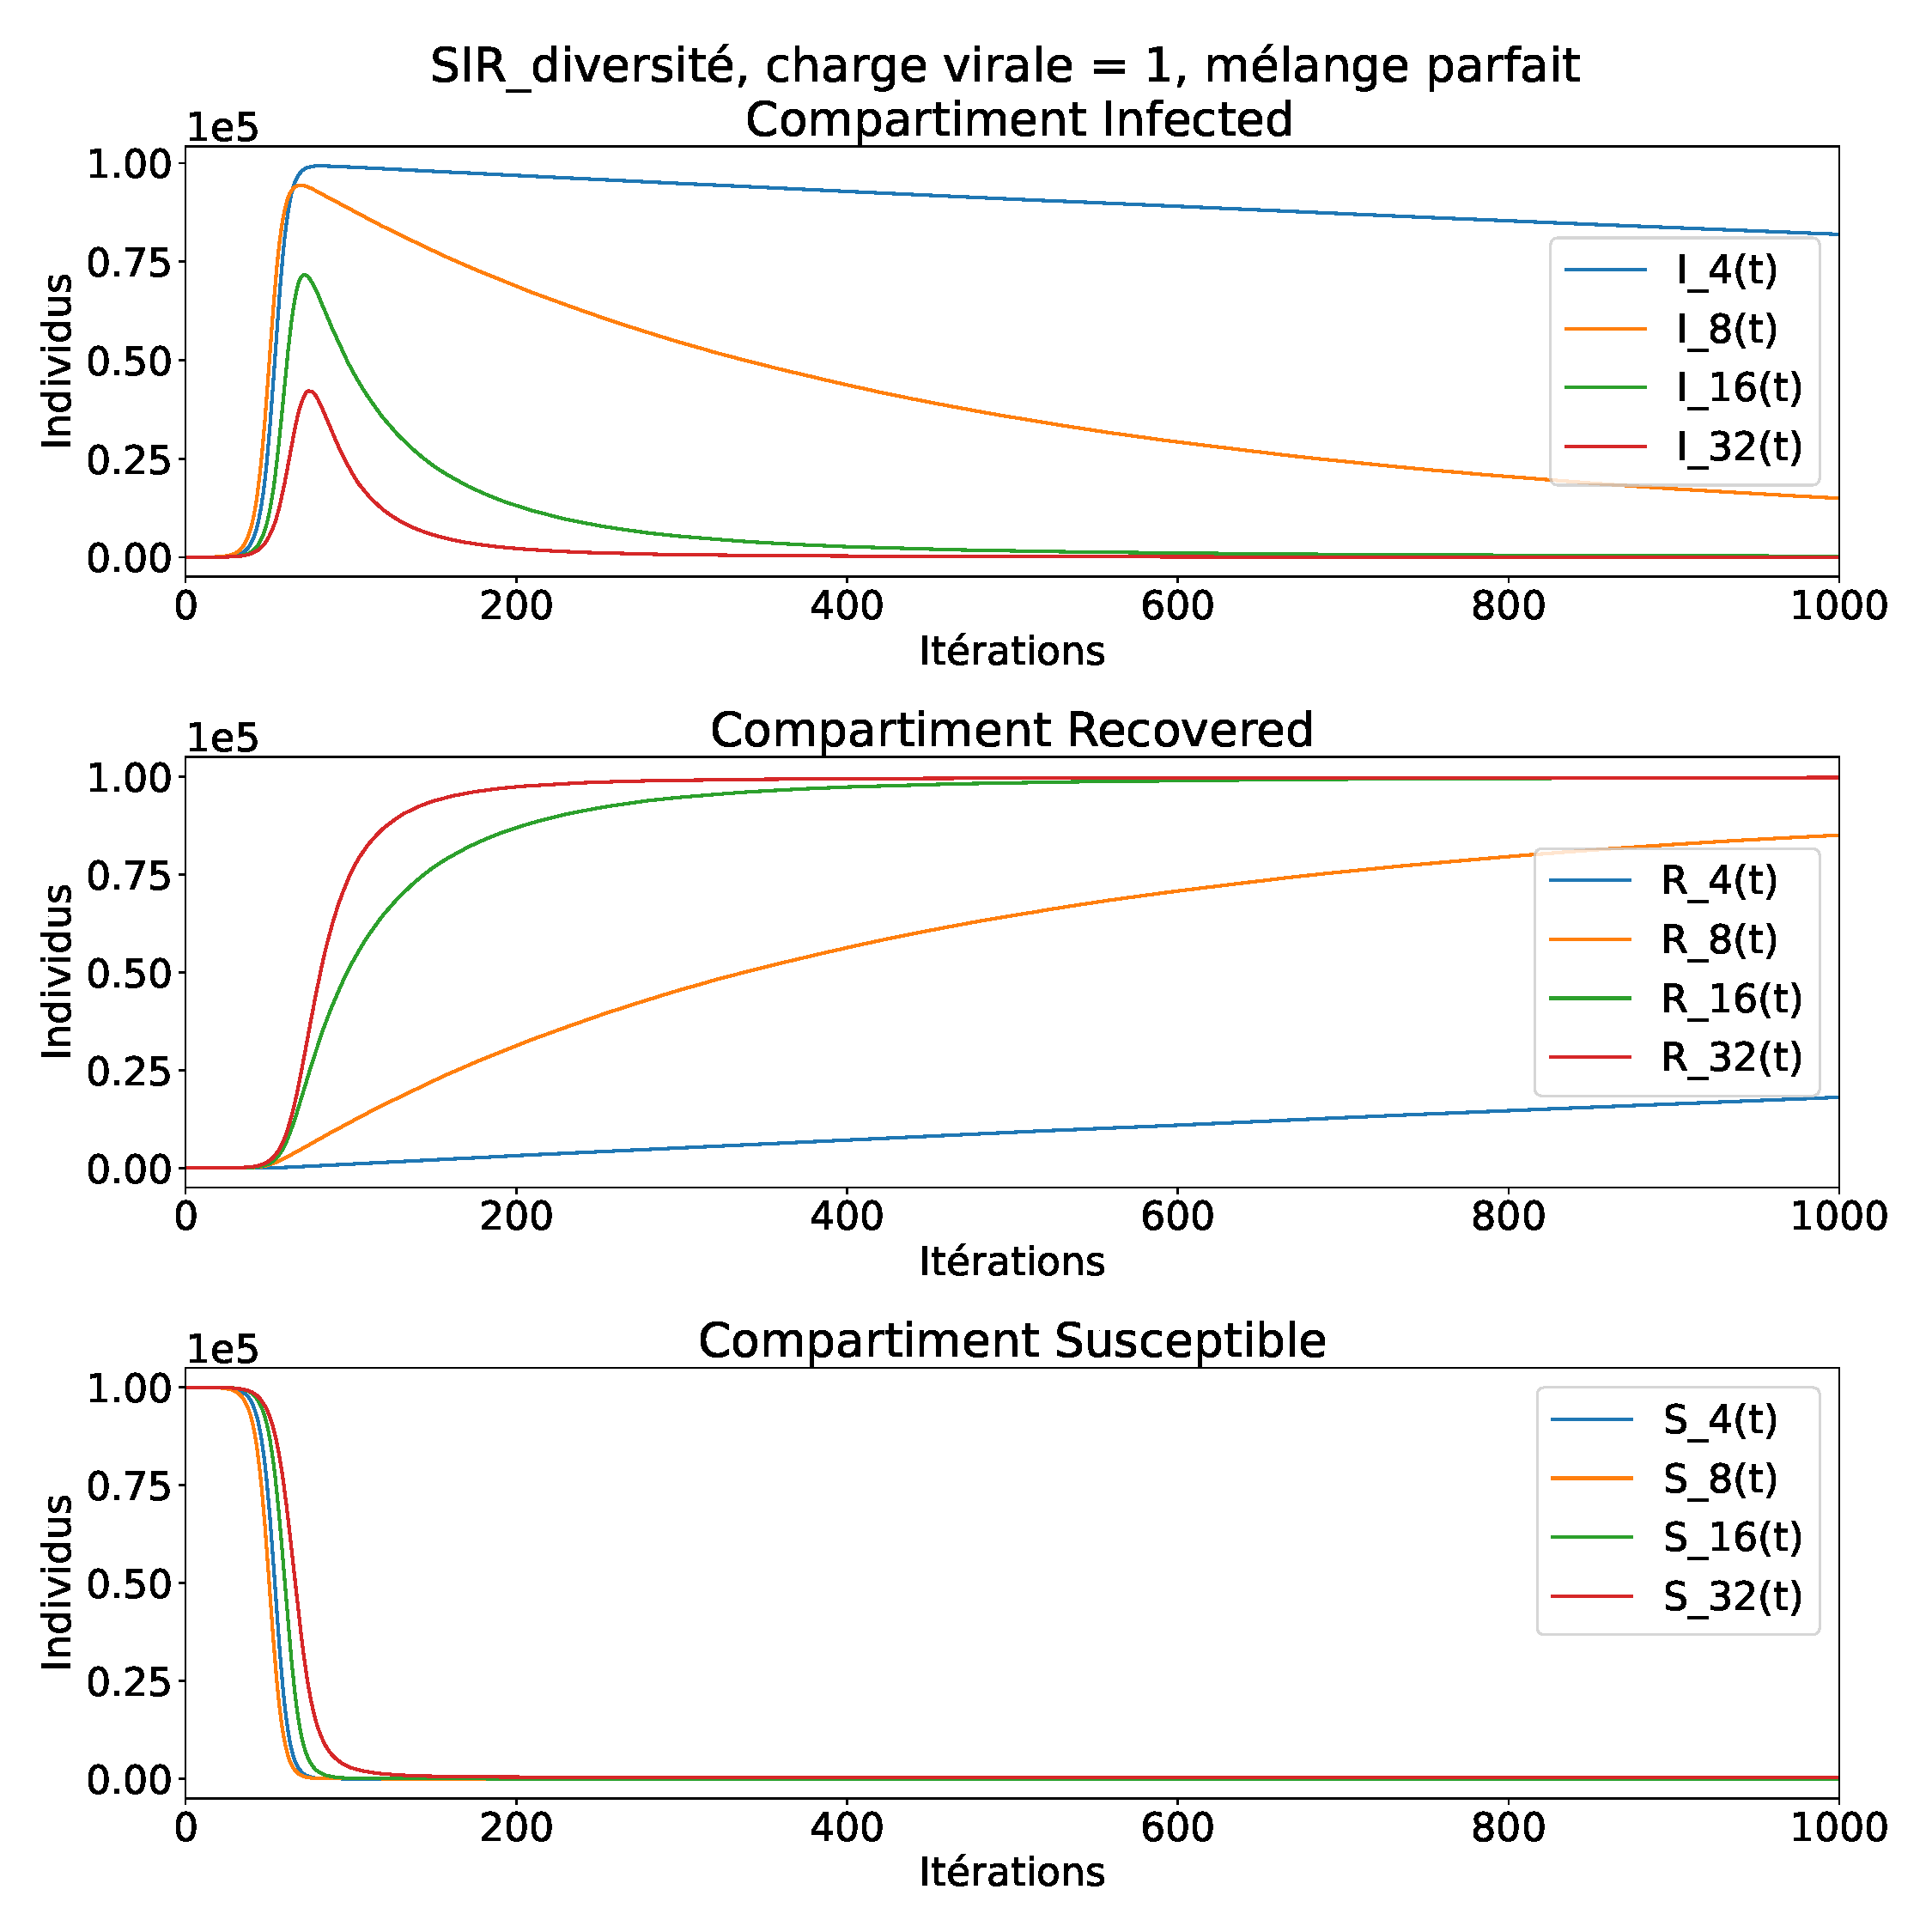
\includegraphics[width=.8\textwidth]{Images/SIR_diversite_mix.pdf}
	\caption[Impacte de la diversité]{Impacte de la diversité d'une population sur une simulation au mélange parfait avec $10^5$ individus et une densité de $1/16$. La première figure montre le compartiment $I$, le second le compartiment $R$ et le dernier le compartiment $S$. Chaque couleur de courbe fait référence à une simulation avec une certaine valeur de diversité notée dans la légende.}
\end{figure}

L'objectif de ce chapitre est d'observer le comportement du système lorsque tous les individus sont contaminés. Un système de densité $1/16$ avec le mélange parfait et une charge virale de $1$ propage très rapidement une pandémie. Il s'agit ici de constater les comportements du système lors des immunisations.\\

La première observation est que pour les $4$ simulations, tous les individus quittent rapidement le compartiment $S$ mais ceci légèrement moins rapidement pour les simulations à forte diversité. Ceci est dû au fait qu'une grande diversité produit des individus s'immunisant très rapidement qui freinent la propagation du pathogène mais l'impact n'est que très léger.\\

La seconde constatation se trouve dans le compartiment $R$. Les individus contaminés s'immunisent plus rapidement dans les systèmes à forte diversité. Ce résultat suit l'intuition car les génomes initiaux avantagent l'agent pathogène et donc réduisent la probabilité pour les individus de s'immuniser. Par conséquent, une forte diversité réduit la compatibilité entre les agents pathogènes et les individus et permettent une immunisation plus rapide.

\section{Taux de pandémies}

Ce chapitre cherche à établir des statistiques concernant des simulations qui ne développent pas de pandémies. L'objectif est que quantifier l'impact de la diversité sur le taux de simulations qui donnent ou ne donnent pas de pandémie. Cette section nécessite des statistiques sur un grand nombre de simulations car nous mesurons des événements qui sont très sensibles aux variations.\\

Toutes les configurations étudiées sont de taille $1264 \times 1264$ avec $10^5$ individus. La charge virale et le nombre de mouvements varie d’une configuration à l’autre. Les valeurs de charge virale étudiées sont : $0.25,0.5,0.75,1$ et les valeurs pour les mouvements sont : $1,10,50$. Pour chacune de ces simulations $4$ niveaux de diversité sont explorés : $4,8,16,32$.\\

Les simulations ont deux conditions d'arrêt. La première arrive lorsque plus aucun individu n'est contaminé et la seconde survient lorsque $10\%$ de la population a été touchées par la pandémie. Nous estimons qu'à partir de $10\%$, les simulations adoptent un comportement déterministe.\\ 

La suite présente des statistiques sur les simulations incluant de la diversité qui n'ont pas développé de pandémie. En effet, nous nous intéressons tout particulièrement aux situations ou une pandémie est évitée. Les données relevées concernant ces simulations sont : le nombre maximum de contaminés simultanément, l'itération de ce maximum, l'itération de fin de simulation (lorsque plus aucun individu n'est contaminé), l'ampleur de la pandémie (nombre de personnes sorties du compartiment $S$) et finalement le taux de simulations qui n'ont pas développé de pandémie parmi les $100$ simulations pour chaque configuration.\\

Un total de $64$ configurations de simulations sont étudiées et pour chacune de ces configurations nous effectuons $100$ run. L'exécution de $100$ simulations pour un ensemble de paramètres permet de calculer le taux d'événements pandémiques ainsi que de relever les caractéristiques des simulations qui ne font pas apparaitre de pandémie.

\begin{table}[H]
	\centering
	\renewcommand{\arraystretch}{0.6}
	\captionsetup{justification=centering}
	\caption[Taux d'échecs : diversité 4]{Résultats moyennées des 100 simulations sur un ensemble de $12$ configurations à diversité $4$. Nous mesurons le taux d'échecs des pandémies ainsi que la taille totale des pandémies qui échouent.\label{tab:grid}}
	\begin{tabular}{@{\extracolsep{\fill} } |c| c| c| c| c|}
		\toprule
		Diversité & charge virale & Mouvements & Echecs & Taille pandémie \\
		\midrule
		4         & 1             & 1          & 0\%  & nan             \\
		\midrule
		4         & 1             & 10         & 0\%  & nan             \\
		\midrule
		4         & 1             & 50         & 0\%  & nan             \\
		\midrule
		4         & 0.75          & 1          & 1\%   & 1               \\
		\midrule
		4         & 0.75          & 10         & 0\%  & nan             \\
		\midrule
		4         & 0.75          & 50         & 0\%  & nan             \\
		\midrule
		4         & 0.5           & 1          & 1\%   & 1               \\
		\midrule
		4         & 0.5           & 10         & 0\%  & nan             \\
		\midrule
		4         & 0.5           & 50         & 0\%  & nan             \\
		\midrule
		4         & 0.25          & 1          & 0\%  & nan             \\
		\midrule
		4         & 0.25          & 10         & 2\%   & 1               \\
		\midrule
		4         & 0.25          & 50         & 0\%  & nan             \\
		\bottomrule
	\end{tabular}
\end{table}

Les taux d'échecs des simulations en diversité $4$ sont dû au fait que l'agent pathogène reste très virulent même avec une distance de Hamming maximale de $4$ dans ces configurations. Par conséquent, presque toutes les simulations finissent sur une pandémie.

\begin{table}[H]
	\centering
	\renewcommand{\arraystretch}{0.6}
	\captionsetup{justification=centering}
	\caption[Statistiques : diversité 4]{Résultats moyennées des 100 simulations sur un ensemble de $12$ configurations à diversité $4$. Nous mesurons le maximum d'individus contaminés simultanément, l'itération de ce maximum ainsi que l'itération de la fin de la simulation. A nouveau, nous ne mesurons que pour les simulations qui ne développent pas de pandémie.\label{tab:grid}}
	\begin{tabular}{@{\extracolsep{\fill} } |c| c| c| c| c| c|}
		\toprule
		Diversité & Charge virale & Mouvements & Max & Itération max & Itération fin \\
		\midrule
		4         & 1             & 1          & nan & nan           & nan           \\
		\midrule
		4         & 1             & 10         & nan & nan           & nan           \\
		\midrule
		4         & 1             & 50         & nan & nan           & nan           \\
		\midrule
		4         & 0.75          & 1          & 1   & 0             & 24            \\
		\midrule
		4         & 0.75          & 10         & nan & nan           & nan           \\
		\midrule
		4         & 0.75          & 50         & nan & nan           & nan           \\
		\midrule
		4         & 0.5           & 1          & nan & nan           & nan           \\
		\midrule
		4         & 0.5           & 10         & nan & nan           & nan           \\
		\midrule
		4         & 0.5           & 50         & nan & nan           & nan           \\
		\midrule
		4         & 0.25          & 1          & nan & nan           & nan           \\
		\midrule
		4         & 0.25          & 10         & 1   & 0             & 4.5           \\
		\midrule
		4         & 0.25          & 50         & nan & nan           & nan           \\
		\bottomrule
	\end{tabular}
\end{table}

Toutes les configurations qui n'ont pas de pandémie déclarée n'ont pas relevé d'informations. Pour les rares simulations à avoir échoué, les échecs se produisent parce que le patient zéro n'est parvenu à contaminer personne.

\begin{table}[H]
	\centering
	\renewcommand{\arraystretch}{0.6}
	\captionsetup{justification=centering}
	\caption[Taux d'échecs : diversité 8]{Résultats moyennées des 100 simulations sur un ensemble de $12$ configurations à diversité $8$. Nous mesurons le taux d'échecs des pandémies ainsi que la taille totale des pandémies qui échouent.\label{tab:grid}}
	\begin{tabular}{@{\extracolsep{\fill} } |c| c| c| c| c|}
		\toprule
		Diversité & charge virale & Mouvements & Echecs & Taille pandémie \\
		\midrule
		8         & 1             & 1          & 1\%   & 1               \\
		\midrule
		8         & 1             & 10         & 0\%  & nan             \\
		\midrule
		8         & 1             & 50         & 0\%  & nan             \\
		\midrule
		8         & 0.75          & 1          & 2\%   & 1               \\
		\midrule
		8         & 0.75          & 10         & 2\%   & 1.5             \\
		\midrule
		8         & 0.75          & 50         & 1\%   & 1               \\
		\midrule
		8         & 0.5           & 1          & 4\%   & 1               \\
		\midrule
		8         & 0.5           & 10         & 2\%   & 1               \\
		\midrule
		8         & 0.5           & 50         & 2\%   & 1               \\
		\midrule
		8         & 0.25          & 1          & 7\%   & 1               \\
		\midrule
		8         & 0.25          & 10         & 4\%   & 1               \\
		\midrule
		8         & 0.25          & 50         & 6\%   & 1               \\
		\bottomrule
	\end{tabular}
\end{table}

Mêmes observations pour les simulations en diversité $8$. Les taux d'échecs sont très faibles et les tailles des pandémies sont minimales sur les simulations qui échouent.

\begin{table}[H]
	\centering
	\renewcommand{\arraystretch}{0.6}
	\captionsetup{justification=centering}
	\caption[Statistiques : diversité 8]{Résultats moyennées des 100 simulations sur un ensemble de $12$ configurations à diversité $8$. Nous mesurons le maximum d'individus contaminés simultanément, l'itération de ce maximum ainsi que l'itération de la fin de la simulation. A nouveau, nous ne mesurons que pour les simulations qui ne développent pas de pandémie.\label{tab:grid}}
	\begin{tabular}{@{\extracolsep{\fill} } |c| c| c| c| c| c|}
		\toprule
		Diversité & Charge virale & Mouvements & Max & Itération max & Itération fin \\
		\midrule
		8         & 1             & 1          & 1   &               & 15            \\
		\midrule
		8         & 1             & 10         & nan & nan           & nan           \\
		\midrule
		8         & 1             & 50         & nan & nan           & nan           \\
		\midrule
		8         & 0.75          & 1          & 1   & 0             & 9.5           \\
		\midrule
		8         & 0.75          & 10         & 1.5 & 5.5           & 12            \\
		\midrule
		8         & 0.75          & 50         & 1   & 0             & 9             \\
		\midrule
		8         & 0.5           & 1          & 1   & 0             & 6.75          \\
		\midrule
		8         & 0.5           & 10         & 1   & 0             & 5             \\
		\midrule
		8         & 0.5           & 50         & 1   & 0             & 16            \\
		\midrule
		8         & 0.25          & 1          & 1   & 0             & 31.43         \\
		\midrule
		8         & 0.25          & 10         & 1   & 0             & 9.25          \\
		\midrule
		8         & 0.25          & 50         & 1   & 0             & 11.5          \\
		\bottomrule
	\end{tabular}
\end{table}

Toutes les simulations en diversité $8$ qui ne donnent pas de pandémies sont dû au fait que le patient zéro n'a contaminé personne et le pathogène meurt trop vite.

\begin{table}[H]
	\centering
	\renewcommand{\arraystretch}{0.6}
	\captionsetup{justification=centering}
	\caption[Taux d'échecs : diversité 16]{Résultats moyennées des 100 simulations sur un ensemble de $12$ configurations à diversité $16$. Nous mesurons le taux d'échecs des pandémies ainsi que la taille totale des pandémies qui échouent.\label{tab:grid}}
	\begin{tabular}{@{\extracolsep{\fill} } |c| c| c| c| c|}
		\toprule
		Diversité & charge virale & Mouvements & Echecs & Taille pandémie \\
		\midrule
		16        & 1             & 1          & 19\%   & 1.32            \\
		\midrule
		16        & 1             & 10         & 10\%   & 1               \\
		\midrule
		16        & 1             & 50         & 0\%  & nan             \\
		\midrule
		16        & 0.75          & 1          & 25\%   & 3.04            \\
		\midrule
		16        & 0.75          & 10         & 13\%   & 1.15            \\
		\midrule
		16        & 0.75          & 50         & 10\%   & 1.1             \\
		\midrule
		16        & 0.5           & 1          & 41\%   & 4.88            \\
		\midrule
		16        & 0.5           & 10         & 14\%   & 1.36            \\
		\midrule
		16        & 0.5           & 50         & 12\%   & 1.17            \\
		\midrule
		16        & 0.25          & 1          & 99\%    & 816.92          \\
		\midrule
		16        & 0.25          & 10         & 33\%   & 1.76            \\
		\midrule
		16        & 0.25          & 50         & 28\%   & 1.32            \\
		\bottomrule
	\end{tabular}
\end{table}

L'impact de la diversité apparait à partir d'une diversité de $16$. Naturellement, le nombre de mouvement impacte grandement l'échec d'une pandémie et ceci est perçu dans les taux d'échecs. Les taux d'échecs de la table au-dessus sont nettement plus élevés que pour les mêmes simulations aux diversités inférieures mais la taille des pandémies reste très faible sauf pour une configuration. Généralement les simulations à cette diversité échouent sans se propager du tout mais la simulation de diversité $16$, charge virale $0.25$ avec un nombre de mouvement de $1$ montre des comportement étonnants.\\

Presque toutes les simulations de cette configuration ont échoué et ceci avec une taille de pandémie moyenne de plus de $816$ individus. C'est pour l'instant la seule configuration à montrer des plus grandes pandémies mais qui finissent quand même par échouer.

\begin{table}[H]
	\centering
	\renewcommand{\arraystretch}{0.6}
	\captionsetup{justification=centering}
	\caption[Statistiques : diversité 16]{Résultats moyennées des 100 simulations sur un ensemble de $12$ configurations à diversité $16$. Nous mesurons le maximum d'individus contaminés simultanément, l'itération de ce maximum ainsi que l'itération de la fin de la simulation. A nouveau, nous ne mesurons que pour les simulations qui ne développent pas de pandémie.\label{tab:grid}}
	\begin{tabular}{@{\extracolsep{\fill} } |c| c| c| c| c| c|}
		\toprule
		Diversité & Charge virale & Mouvements & Max   & Itération max & Itération fin \\
		\midrule
		16        & 1             & 1          & 1.21  & 1.37          & 12.37         \\
		\midrule
		16        & 1             & 10         & 1     & 0             & 5.3           \\
		\midrule
		16        & 1             & 50         & nan   & nan           & nan           \\
		\midrule
		16        & 0.75          & 1          & 2.32  & 8.32          & 31.52         \\
		\midrule
		16        & 0.75          & 10         & 1.15  & 0.46          & 7.23          \\
		\midrule
		16        & 0.75          & 50         & 1.1   & 0.2           & 5.4           \\
		\midrule
		16        & 0.5           & 1          & 2.17  & 16.90         & 51.34         \\
		\midrule
		16        & 0.5           & 10         & 1.36  & 0.71          & 7.21          \\
		\midrule
		16        & 0.5           & 50         & 1.17  & 0.17          & 14.5          \\
		\midrule
		16        & 0.25          & 1          & 28.05 & 989.47        & 2632.66       \\
		\midrule
		16        & 0.25          & 10         & 1.58  & 6.91          & 25.88         \\
		\midrule
		16        & 0.25          & 50         & 1.21  & 3.07          & 15.82         \\
		\bottomrule
	\end{tabular}
\end{table}

De toutes les simulations qui ont échoué, seule une persiste et parvient à contaminer un maximum de $28$ individus en moyenne et finit par s'achever à l'itération $2632$ en moyenne.

\begin{table}[H]
	\centering
	\renewcommand{\arraystretch}{0.6}
	\captionsetup{justification=centering}
	\caption[Taux d'échecs : diversité 32]{Résultats moyennées des 100 simulations sur un ensemble de $12$ configurations à diversité $32$. Nous mesurons le taux d'échecs des pandémies ainsi que la taille totale des pandémies qui échouent.\label{tab:grid}}
	\begin{tabular}{@{\extracolsep{\fill} } |c| c| c| c| c|}
		\toprule
		Diversité & charge virale & Mouvements & Echecs & Taille pandémie \\
		\midrule
		32        & 1             & 1          & 100\%    & 18.02           \\
		\midrule
		32        & 1             & 10         & 28\%   & 1.36            \\
		\midrule
		32        & 1             & 50         & 0\%  & nan             \\
		\midrule
		32        & 0.75          & 1          & 100\%    & 13.46           \\
		\midrule
		32        & 0.75          & 10         & 33\%   & 1.97            \\
		\midrule
		32        & 0.75          & 50         & 24\%   & 1.63            \\
		\midrule
		32        & 0.5           & 1          & 100\%    & 10.98           \\
		\midrule
		32        & 0.5           & 10         & 51\%   & 2.31            \\
		\midrule
		32        & 0.5           & 50         & 57\%   & 1.58            \\
		\midrule
		32        & 0.25          & 1          & 100\%    & 4.56            \\
		\midrule
		32        & 0.25          & 10         & 100\%    & 180.12          \\
		\midrule
		32        & 0.25          & 50         & 81\%   & 3.23            \\
		\bottomrule
	\end{tabular}
\end{table}

Finalement les configurations en diversité $32$ montrent les taux les plus faibles. Toutes les configurations à $1$ mouvement n'ont donné aucune pandémie et ceci contrairement aux mêmes configurations à diversité inférieure.

\begin{table}[H]
	\centering
	\renewcommand{\arraystretch}{0.6}
	\captionsetup{justification=centering}
	\caption[Statistiques : diversité 32]{Résultats moyennées des 100 simulations sur un ensemble de $12$ configurations à diversité $32$. Nous mesurons le maximum d'individus contaminés simultanément, l'itération de ce maximum ainsi que l'itération de la fin de la simulation. A nouveau, nous ne mesurons que pour les simulations qui ne développent pas de pandémie.\label{tab:grid}}
	\begin{tabular}{@{\extracolsep{\fill} } |c| c| c| c| c| c|}
		\toprule
		Diversité & Charge virale & Mouvements & Max  & Itération max & Itération fin \\
		\midrule
		32        & 1             & 1          & 5.1  & 40.09         & 104.05        \\
		\midrule
		32        & 1             & 10         & 1.25 & 0.68          & 6.32          \\
		\midrule
		32        & 1             & 50         & nan  & nan           & nan           \\
		\midrule
		32        & 0.75          & 1          & 3.99 & 37.93         & 103.11        \\
		\midrule
		32        & 0.75          & 10         & 1.39 & 1.03          & 9.03          \\
		\midrule
		32        & 0.75          & 50         & 1.46 & 1.54          & 7.46          \\
		\midrule
		32        & 0.5           & 1          & 3    & 34.47         & 100.25        \\
		\midrule
		32        & 0.5           & 10         & 1.65 & 4.63          & 14.31         \\
		\midrule
		32        & 0.5           & 50         & 1.29 & 2.86          & 10.91         \\
		\midrule
		32        & 0.25          & 1          & 2.11 & 19.64         & 51.55         \\
		\midrule
		32        & 0.25          & 10         & 7.12 & 145.94        & 245.44        \\
		\midrule
		32        & 0.25          & 50         & 1.88 & 10.67         & 26.51         \\
		\bottomrule
	\end{tabular}
\end{table}

A nouveau, une grande majorité des configurations à diversité $32$ ne montrent que des pandémies qui naissent avec des maximums de contaminés de l'ordre d'une dizaine d'individus et une fin de simulations très rapide.

\section{Pandémies partielles}

Jusqu'à présent, le modèle n'a pas montré de simulations qui donnent des pandémies qui contaminent une portion non nulle de la population sans pour autant contaminer tout le monde. Certaines configurations font apparaitre ce type d'événement avec certains paramètres qui favorisent la présence de pandémies partielles. Plus particulièrement, deux conditions favorisent la présence de ces phénomènes. Le premier est une densité faible ce qui ralenti la propagation de la pandémie et peut donc permettre sa disparition. La seconde est un nombre de mouvements élevé ou le mélange parfait.\\

Une faible densité d'un système permet d'observer des pandémies avec peu de contaminés simultanément et qui évoluent lentement. Dû au peu de contaminés simultanés il est possible que tous les individus contaminés s'immunisent et ne parviennent pas à contaminer davantage d'individus. La méthode de mouvement joue aussi un rôle dans l'observation de ces phénomènes. Généralement, plus le mélange des individus est bon, plus on peut observer de pandémies partielles et ceci est dû au fait de l'immunisation collective.\\

Toutes les simulations effectuées durant la totalité du travail n’ont que rarement donné de pandémies partielles. L’apparition de ces phénomènes de manière partielle nécessite d’être proche d’une limite, c’est-à-dire dans une situation instable de propagation. D’après les essais effectués, une simulation aux mouvements multiple peine à donner de pandémies partielles. 

\begin{figure}[h]
	\centering
	\captionsetup{justification=centering}
	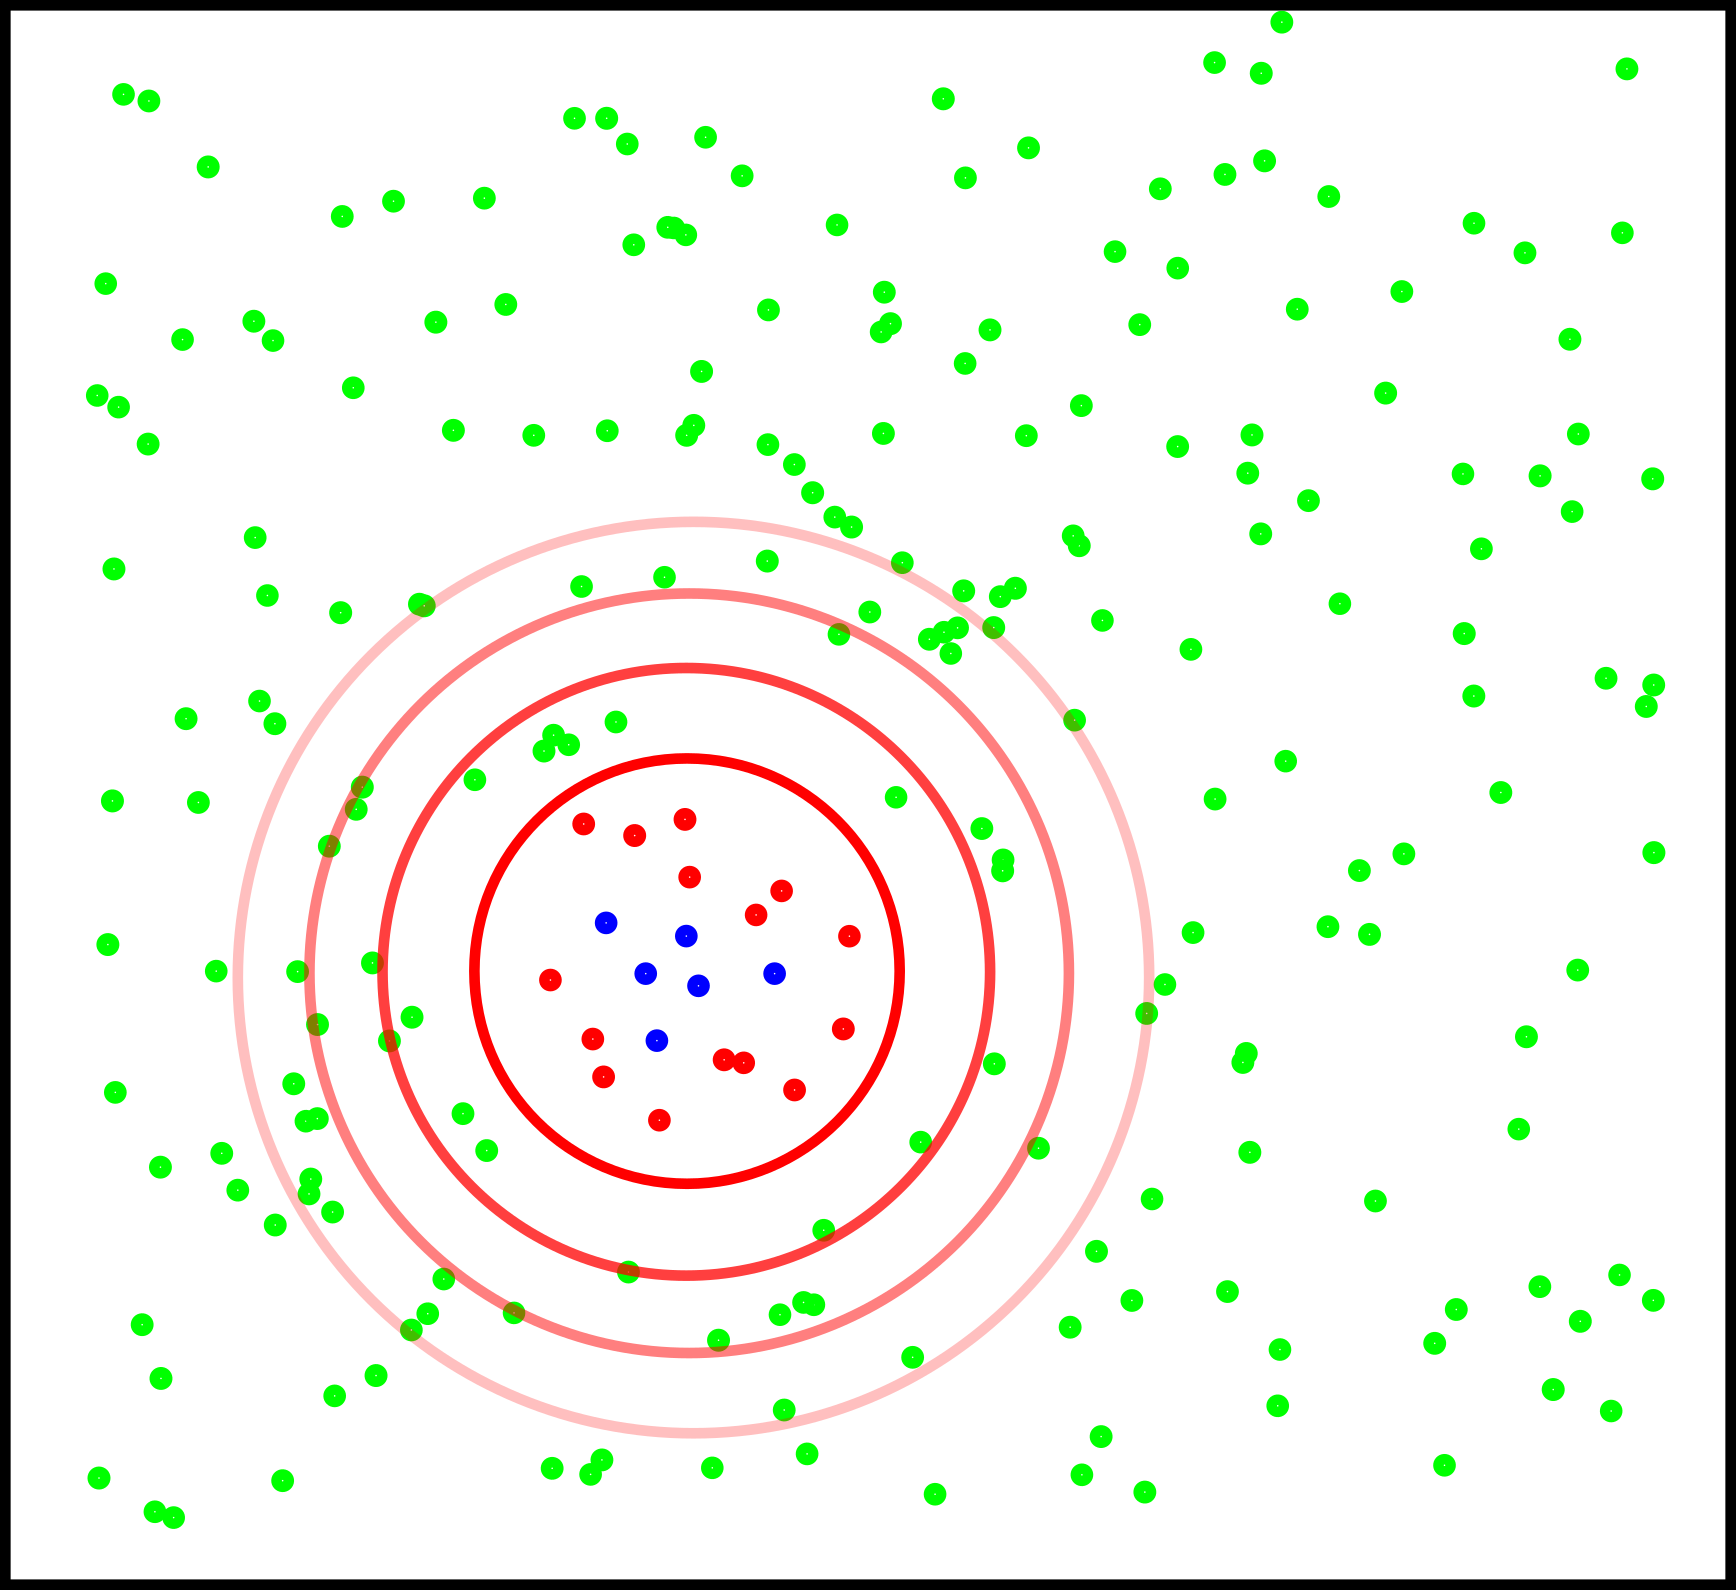
\includegraphics[width=.5\textwidth]{Images/vague_propagation.png}
	\caption[Vague de propagation]{Représentation du fonctionnement du modèle pour des simulations aux multiples mouvements. En bleu nous avons les individus immunisés, en rouge les individus contaminés et en vert les individus sains. Les cercles rouges représentent la "vague" de propagation de la pandémie.}
\end{figure} 

L’image ci-dessus montre une situation de propagation de pandémie dans une configuration aux multiples mouvements. Si le nombre de mouvements défini est trop faible, le système peut être représenté sous cette forme avec $3$ zones distinctes. La première zone est les individus en bleu qui se sont immunisé au pathogène, la seconde est la “vague” avec les individus contaminés qui en contaminent d’autres et finalement la troisième est le reste du système uniformément rempli d’individus sains.\\ 

Le problème de ce mode de fonctionnement est que la pandémie se propage telle une vague ou une onde. Cette propagation se produit dans la troisième zone qui est un milieu uniforme. Par conséquent les simulations finissent généralement de deux manières différentes. La première est que la vague ne parvient pas à se propager et le pathogène meurt très tôt dans la simulation. La deuxième est que la vague parvienne à se propager. Si l'événement se déclare et étant donnée l'uniformité de la zone $3$ alors la panémie est totale.\\ 

Pour contourner ce problème et observer des pandémies partielles nous utilisons le mélange parfait. La différence est que la zone $3$ n’est plus uniformément remplie d’individus sains mais se mélange avec des individus immunisés. Par conséquent, ces individus immunisés bloquent la propagation et permettent de faire apparaitre des pandémies partielles. C’est un principe d’immunité collective.\\ 

Les simulations étudiées sont des configurations de taille $2000 \times 2000$ (densité $1/40$) au mélange parfait avec une charge virale variant de : $1, 0.75, 0.5$ et avec une diversité variant de : $4,8,16,20,24,28,32,36,40,1000$. Pour chacune des $30$ configurations, un total de $100$ exécutions ont été effectuées et les résultats moyennés. La seule mesure prise est la taille totale de la pandémie, c'est-à-dire le compte de tous les individus qui ont quitté le compartiment $S$.\\

Les génomes sont codés sur $32$ bits et sont initialement identiques pour tous les acteurs du système. La diversité permet de faire dévier les génomes des individus afin de réduire la compatibilité avec l'agent pathogène (ceci le rend moins virulent). La valeur de diversité d'une configuration détermine le nombre de complémentations aléatoire sur la séquence de génome et ce nombre n'est pas borné. Par conséquent, une diversité de $32$ sur des génomes de $32$ ne signifie pas que la diversité des individus est maximale. Les résultats suivants montrent l'impact de ces valeurs de diversité sur l'ampleur des pandémies.

\begin{table}[H]
	\centering
	\renewcommand{\arraystretch}{0.6}
	\captionsetup{justification=centering}
	\caption[Taille pandémies, charge virale = 1]{Simulations mesurant la taille de la pandémie pour un ensembles de configurations à charge virale = 1. La taille de pandémie représente tous les individus qui ont quitté le compartiment $S$ lors de la simulation.\label{tab:grid}}
	\begin{tabular}{@{\extracolsep{\fill} } |c| c| c|}
		\toprule
		Charge virale & Diversité & Taille pandémie \\
		\midrule
		1             & 4         & 100000          \\
		\midrule
		1             & 8         & 100000          \\
		\midrule
		1             & 16        & 99922.68        \\
		\midrule
		1             & 20        & 98699.38        \\
		\midrule
		1             & 24        & 95390.15        \\
		\midrule
		1             & 28        & 91217.14        \\
		\midrule
		1             & 32        & 87863.19        \\
		\midrule
		1             & 36        & 85895.91        \\
		\midrule
		1             & 40        & 85180.41        \\
		\midrule
		1             & 1000      & 86335.36        \\
		\bottomrule
	\end{tabular}
\end{table}

Les premiers résultats montrent qu'une plus grande diversité réduit la taille des pandémies. Le minimum atteint sur ces configurations est à une diversité de $40$. Une diversité trop élevée est moins efficace car nous avons simplement des génomes aléatoires et non plus des génomes déviants de l'agent pathogène.

\begin{table}[H]
	\centering
	\renewcommand{\arraystretch}{0.6}
	\captionsetup{justification=centering}
	\caption[Taille pandémies, charge virale = 0.75]{Simulations mesurant la taille de la pandémie pour un ensembles de configurations à charge virale = 0.75. La taille de pandémie représente tous les individus qui ont quitté le compartiment $S$ lors de la simulation.\label{tab:grid}}
	\begin{tabular}{@{\extracolsep{\fill} } |c| c| c|}
		\toprule
		Charge virale & Diversité & Taille pandémie \\
		\midrule
		0.75          & 4         & 100000          \\
		\midrule
		0.75          & 8         & 100000          \\
		\midrule
		0.75          & 16        & 99519.62        \\
		\midrule
		0.75          & 20        & 95731.53        \\
		\midrule
		0.75          & 24        & 88009.51        \\
		\midrule
		0.75          & 28        & 79550.08        \\
		\midrule
		0.75          & 32        & 73206.16        \\
		\midrule
		0.75          & 36        & 69406.5         \\
		\midrule
		0.75          & 40        & 68092.52        \\
		\midrule
		0.75          & 1000      & 70344.02        \\
		\bottomrule
	\end{tabular}
\end{table}

Réduire la charge virale diminue la taille des pandémies. La contagion de l'agent pathogène étant inférieure, la propagation est réduite. 

\begin{table}[H]
	\centering
	\renewcommand{\arraystretch}{0.6}
	\captionsetup{justification=centering}
	\caption[Taille pandémies, charge virale = 0.5]{Simulations mesurant la taille de la pandémie pour un ensembles de configurations à charge virale = 0.5. La taille de pandémie représente tous les individus qui ont quitté le compartiment $S$ lors de la simulation.\label{tab:grid}}
	\begin{tabular}{@{\extracolsep{\fill} } |c| c| c|}
		\toprule
		Charge virale & Diversité & Taille pandémie \\
		\midrule
		0.5           & 4         & 100000          \\
		\midrule
		0.5           & 8         & 100000          \\
		\midrule
		0.5           & 16        & 96823.41        \\
		\midrule
		0.5           & 20        & 84180.41        \\
		\midrule
		0.5           & 24        & 64485.21        \\
		\midrule
		0.5           & 28        & 43646.63        \\
		\midrule
		0.5           & 32        & 23020.03        \\
		\midrule
		0.5           & 36        & 11854.48        \\
		\midrule
		0.5           & 40        & 7983.12         \\
		\midrule
		0.5           & 1000      & 11401.21        \\
		\bottomrule
	\end{tabular}
\end{table}

Finalement les mesures en charge virale = 0.5 ont donnée des pandémies très petites avec un minimum à moins de $8000$ individus touchés. 
